\documentclass{article} % For LaTeX2e
\usepackage{nips15submit_e,times}
\usepackage{Style/thesis}

%\documentstyle[nips14submit_09,times,art10]{article} % For LaTeX 2.09


\title{Reinforcement Learning For Systematic Trading}


\author{%
Pierpaolo G. Necchi\\
Mathematical Engineering\\
Politecnico di Milano\\
Milano, IT 20123 \\
\texttt{pierpaolo.necchi@gmail.com}
}


\newcommand{\fix}{\marginpar{FIX}}
\newcommand{\new}{\marginpar{NEW}}

\nipsfinalcopy % Uncomment for camera-ready version

\begin{document}


\maketitle

\begin{abstract}
TODO
\end{abstract}

\section{Introduction}
\label{sec:introduction}

The trading pit of a stock exchange is often imagined by outsiders as a frenzy place, with telephones constantly ringing and traders shouting orders across the room at a frenetic rhythm. This was probably the reality thirty years ago, when open outcry was still the main communication system between pit traders. Since then the floors have become more and more quiet as the majority of the orders moved to electronic trading systems. Notwithstanding, investment decisions were still made by humans who could now execute their orders without passing through the pit traders. In the last decade, the markets have witnessed the arrival of automated trading systems (ATS), that can make investment decisions in a fully automatized way at speeds with orders of magnitude greater than any human equivalent. In 2014, more than $75\%$ of the stock shares traded on United States exchanges were originated from ATS orders and this amount kept growing since then. Quantitative hedge funds, such as Renaissance Technologies, D.E. Shaw, Citadel and many others, are employing mathematicians, physicists and other scientists to develop algorithms able to automatically extract trading signals from large amount of data. These algorithms are typically based on advanced statistics, signal processing, machine learning and many other fields of mathematics. However, few of these hedge funds are keen on publishing their profit-generating ``secret sauce'' and not much can be found in the literature. In this project we develop an automated trading algorithm based on \emph{Reinforcement Learning} (RL), a branch of \emph{Machine Learning} (ML) which has recently been in the spotlight for being at the core of the system who beat the Go world champion in a 5-match series \cite{silver2016mastering}. This document is organized as follows. In Section \ref{sec:basics_reinforcement_learning} we introduce the basic concepts of RL and present two learning algorithms that allow two determine an approximation for the optimal policy of a sequential decision problem. In section \ref{sec:application_to_systematic_trading} we discuss the asset allocation problem from a mathematical point of view and show how these learning algorithms can be applied in this setting. In Section \ref{sec:python_prototype} we start discussing the implementation of the model in Python, which has been used during the prototyping phase. In Section \ref{sec:c++_implementation} we discuss a more efficient C++ implementation. 
In Section \ref{sec:execution_pipeline} we describe the execution pipeline used to run the learning experiment. In Section \ref{sec:numerical_results} we present the numerical results for a synthetic asset, whose price follows a particular stochastic process. In Section \ref{sec:conclusion} we conclude with some final remarks and we discuss some possible research directions. 

\clearpage
\section{Basics of Reinforcement Learning}
\label{sec:basics_reinforcement_learning}

\emph{Reinforcement Learning} (RL) is a general class of algorithms in the field of \emph{Machine Learning} (ML) that allows an agent to learn how to behave in a stochastic and possibly unknown environment, where the only feedback consists of a scalar reward signal \cite{sutton1998introduction}. The goal of the agent is to learn by trial-and-error which actions maximize his long-run rewards. However, since the environment evolves stochastically and may be influenced by the actions chosen, the agent must balance his desire to obtain a large immediate reward by acting greedily and the opportunities that will be available in the future. Thus, RL algorithms can be seen as computational methods to solve sequential decision problems by directly interacting with the environment.\\

\subsection{Markov Decision Processes}
\label{sec:markov_decision_processes}
Sequential decision problems are typically formalized using \emph{Markov Decision Processes} (MDP). An MDP is a stochastic dynamical system specified by the tuple $<\S, \A, \calP, \calR, \gamma>$, where $(\S, \calS)$ is a measurable state space, $(\A, \calA)$ is a measurable action space, $\calP: \S \times \A \times \calS \to \R$ is a Markov transition kernel, $\calR: \S \times \A \to \R$ is a reward function and $0 < \gamma < 1$ is the discount factor. Suppose that at time $t$ the system is in state $S_t = s$ and that the agent takes action $A_t = a$, then, regardless of the previous history of the system, the probability to find the system in a state belonging to $B\in\calS$ at time $t+1$ is given by 
\begin{equation}
	\calP(s, a, B) = \P{S_{t+1} \in B | S_t = s, A_t = a}
\end{equation}
Following this random transition, the agent receives a stochastic reward
$R_{t+1}$. The reward function $\calR(s, a)$ gives the expected reward
obtained when action $a$ is taken in state $s$, i.e. 
\begin{equation}
	\calR(s, a) = \E{R_{t+1} | S_t = s, A_t = a}
\end{equation}
This feedback mechanism between the environment and the agent is illustrated in Figure \ref{fig:sequential_decision_problem}. At any time step, the agent selects his actions according to a certain policy $\pi: \S \times \calA \to \R$ such that for every $s \in \S$, $C \mapsto \pi(s,C)$ is a probability distribution over $(\A, \calA)$. Hence, a policy $\pi$ and an initial state $s_0 \in \S$ determine a random state-action-reward sequence ${\{(S_t, A_t, R_{t+1})\}}_{t\geq 0}$ with values on $\S \times \A \times \R$.
\begin{figure}[t]
	\centering
	\begin{tikzpicture}[node distance = 6em, auto, thick]
		\node [block] (Agent) {Agent};
		\node [block, below of=Agent] (Environment) {Environment};		    
		\path [line] (Agent.0) --++ (4em,0em) |- node [near start]{Action $a_t$} (Environment.0);
		\path [line] (Environment.190) --++ (-6em,0em) |- node [near start]{State  $s_{t}$} (Agent.170);
		\path [line] (Environment.170) --++ (-4.25em,0em) |- node [near start, right] {Reward $r_{t+1}$} (Agent.190);
	\end{tikzpicture}
	\caption{Agent-environment interaction in sequential decision problems.}
	\label{fig:sequential_decision_problem}
\end{figure}
In an infinite horizon task, the agent's performance is typically measured as the total discounted reward obtained following a specific policy
\begin{equation}
	G_t = \sum^{\infty}_{t=0} \gamma^t R_{t+k+1} 
\end{equation}
Since this gain is stochastic, the agent considers its expected value, which is typically called \emph{state-value function}
\begin{equation}
	V_\pi(s) = \E[\pi]{G_t|S_t = s}
\end{equation}
where the subscript in $\mathbb{E}_{\pi}$ indicates that all the actions are selected according to policy $\pi$. The state-value function measures how good it is for the agent to be in a given state and follow a certain policy. Similarly, we introduce the \emph{action-value function}
\begin{equation}
	Q_\pi(s,a) = \E[\pi]{G_t|S_t = s, A_t = a}
\end{equation}
We have the following relationship between $V_\pi$ and $Q_\pi$
\begin{equation}
	V_\pi(s) = \int_\A \pi(s,a) Q_\pi(s,a) da
\end{equation}
Almost all reinforcement learning algorithms are designed to estimate these 
value functions and are typically based on the Bellman equations.
\begin{equation}
	V_\pi(s) = \calR_\pi(s) + \gamma T_\pi V_\pi(s)	
	\label{eq:bellman_expectation_eq_V}
\end{equation}
\begin{equation}
		Q_\pi(s,a) = \calR(s,a) + \gamma T_a V_\pi(s)
		\label{eq:bellman_expectation_eq_Q}
\end{equation}
where we denoted by $T_a$ (resp. $T_\pi$) the transition operator for action 
$a$ (resp. for policy $\pi$)
\begin{equation}
	T_a F(s) = \E{F(S_{t+1})|S_t = s, A_t = a} = \int_\S \calP(s, a, s') F(s') ds'
\end{equation}
\begin{equation}
	T_\pi F(s) = \E[\pi]{F(S_{t+1})|S_t = s} = \int_\A \pi(s,a) \int_\S \calP(s,a,s') F(s') ds'	da
\end{equation}
These equations can be rewritten as fixed-point equations which, under some formal assumptions on the reward functions, admit a unique solution by the contraction mapping theorem. The agent's goal is to select a policy $\pi_*$ that maximizes his expected return in all possible states. Such a policy is called \emph{optimal} and the corrisponding value functions are called \emph{Optimal State-Value Function}
\begin{equation}
	V_*(s) = \sup_\pi V_\pi(s)
\end{equation}
and \emph{Optimal Action-Value Function}
\begin{equation}
	Q_*(s,a) = \sup_\pi Q_\pi(s,a)
\end{equation}
The optimal value functions satisfy the following Bellman equations.
\begin{equation}
	V_*(s) = \sup_a Q_*(s,a) = \sup_a \left\{\calR(s,a) + \gamma T_a V_*(s)\right\}
\end{equation}
\begin{equation}
	\begin{split}
		Q_*(s,a) &= \calR(s,a) + \gamma T_a V_*(s)\\
			 &= \calR(s,a) + \gamma \int_\S \calP(s,a,s') \sup_{a'} Q_*(s', a') ds'
	\end{split}
\end{equation}
Again, these are fixed-point equations for which the existence and uniqueness of a solution is guaranteed by the contraction mapping theorem. Given the optimal action-value function $Q_*$, an optimal policy is obtained by selecting in each state the action with maximizes $Q_*$
\begin{equation}
	a_* = \argsup_a Q_*(s,a)
\end{equation}
This greedy policy is deterministic and only depends on the current state of the system.

\subsection{Policy Gradient Methods}
The standard way to solve MDPs is through dynamic programming, which simply consists in solving the Bellman fixed-point equations discussed in the previous chapter. Following this approach, the problem of finding the optimal policy is transformed into the problem of finding the optimal value function. However, apart from the simplest cases where the MDP has a limited number of states and actions, dynamic programming becomes computationally infeasible. Moreover, this approach requires complete knowledge of the Markov transition kernel and of the reward function, which in many real-world applications might be unknown or too complex to use. \emph{Reinforcement Learning} (RL) is a subfield of Machine Learning which aims to turn the infeasible dynamic programming methods into practical algorithms that can be applied to large-scale problems. RL algorithms are based on two key ideas: the first is to use samples to compactly represent the unknown dynamics of the controlled system. The second idea is to use powerful function approximation methods to compactly estimate value functions and policies in high-dimensional state and action spaces. In this section we will only focus on a particular class of algorithms called \emph{Policy Gradient Methods}, which have proved successful in many applications. For a more complete introduction to RL, the reader may consult \cite{sutton1998introduction}, \cite{szepesvari2010algorithms} or \cite{wiering2012reinforcement}.\\
In \emph{policy gradient methods} \cite{peters2008reinforcement}, the optimal policy is approximated using a parametrized policy $\pi: \S \times \calA \times \Theta \to \R$ such that, given a parameter vector $\theta \in \Theta \subseteq \R^{D_\theta}$, $\pi(s, B; \theta) = \pi_\theta(s, B)$ gives the probability of selecting an action in $B \in \calA$ when the system is in state $s \in \S$.
The general goal of policy optimization in reinforcement learning is to
optimize the policy parameters $\theta \in \Theta$ so as to maximize a certain
objective function $J: \Theta \to \R$
\begin{equation}
	\theta^* = \argmax_{\theta \in \Theta} J(\theta)
\end{equation}
In the following, we will focus on gradient-based and model-free methods that exploit
the sequential structure of the the reinforcement learning problem. The idea of
policy gradient algorithms is to update the policy parameters using the gradient ascent direction of the objective function
\begin{equation}
	\theta_{k+1} = \theta_k + \alpha_k \nabla_\theta J\left(\theta_k\right)
\end{equation}
where $\{\alpha_k\}_{k\geq 0}$ is a sequence of learning rates. Typically, the
gradient of the objective function is not known and its approximation is the key component of every policy gradient algorithm. It is a well-know result from stochastic optimization \cite{kushner2003stochastic} that, if the gradient estimate is unbiased and the learning rates satisfy the \emph{Robbins-Monro conditions}
\begin{equation}
	\sum_{k=0}^\infty \alpha_k = \infty \;\;\;\;\;\; \sum^{\infty}_{k=0}
	\alpha_k^2 < \infty 
\end{equation}
the learning process is guaranteed to converge at least to a local optimum of
the objective function. In an episodic environment where the system always starts from an initial state $s_0$, the typical objective function is the start value.
\begin{equation}
	J_{\text{start}}(\theta) = V_{\pi_\theta}(s_0) = \E[\pi_\theta]{G_0 |
 S_0 = s_0}
\end{equation}
In a continuing environment, where no terminal state exists and the task might go on forever, it is common to use either the average value 
\begin{equation}
	J_{\text{avV}}(\theta) = \E[S \sim d^{\theta}]{V_{\pi_\theta}(S)} = \int_\S
	d^{\theta}(s) V_{\pi_\theta}(s) ds
\end{equation}
where $d^\theta$ is the stationary distribution of the Markov chain induced by $\pi_\theta$. Alternatively, one may use the average reward per time step
\begin{equation}
	J_{\text{avR}}(\theta) = \rho(\theta) = \E[\substack{S \sim d^{\theta}\\A \sim \pi_\theta}]{\calR(S,A)} 
	= \int_\S d^{\theta}(s) \int_\A \pi_\theta(s,a) \calR(s,a) da ds
\end{equation}
Luckily, the same methods apply with minor changes to the three objective functions. 

\subsubsection{Policy Gradient Theorem}
The \emph{policy gradient theorem} \cite{sutton1999policy} shows that the gradient can be rewritten in a form suitable for estimation from experience aided by an approximate action-value or advantage function.
\begin{theorem}[Policy Gradient]
\label{thm:risk_neutral_policy_gradient}
	Let $\pi_\theta$ be a differentiable policy. The policy gradient for the average reward formulation is given by
	\begin{equation}
		\nabla_\theta \rho(\theta) =
		\E[\substack{S \sim d^\theta\\A \sim \pi_\theta}]{\nabla_\theta\log
		\pi_\theta(S,A) Q_{\theta}(S, A)}
	\end{equation}
	where $d^\theta$ is the stationary distribution of the Markov chain induced by $\pi_\theta$. The policy gradient for the start value formulation is given by
	\begin{equation}
		\nabla_\theta J_{\text{start}}(\theta) =
		\E[\substack{S \sim d_\gamma^\theta(s_0, \cdot)\\A \sim \pi_\theta}]{\nabla_\theta\log
		\pi_\theta(S,A) Q_{\theta}(S, A)}
	\end{equation}
	where $d_\gamma^\theta(s_0, \cdot)$ is the $\gamma$-discounted visiting distribution over states starting from the initial state $s_0$ and following policy $\pi_\theta$
		\begin{equation}
			d_\gamma^\theta(s, x) = \sum_{k=0}^{\infty} \gamma^k \calP_\theta^{(k)}(s, x)
		\end{equation}
\end{theorem}
Let us notice that we can subtract a state-dependent baseline from the action-value function without changing the value of the expectation, indeed
\begin{equation*}
	\begin{split}
	\E[\substack{S \sim d^\theta\\A \sim \pi_\theta}]{\nabla_\theta\log
			\pi_\theta(S,A) B_\theta(S)} 
	&= \int_\S d^\theta(s) \int_\A \pi_\theta(s,a) \nabla_\theta\log
				\pi_\theta(s,a) B_\theta(s) da ds\\
	&= \int_\S d^\theta(s)  B_\theta(s) \int_\A \nabla_\theta \pi_\theta(s,a) da ds\\
	&= \int_\S d^\theta(s)  B_\theta(s)  \nabla_\theta  \underbrace{\int_\A  \pi_\theta(s,a) da}_{= 1} ds = 0
	\end{split}
\end{equation*}
Hence, the policy gradient theorem can be rewritten as 
\begin{equation}
\label{eq:pg_theorem_baseline}
	\nabla_\theta \rho(\theta) =
	\E[\substack{S \sim d^\theta\\A \sim \pi_\theta}]{\nabla_\theta\log
	\pi_\theta(S,A) \left(Q_{\pi_\theta}(S, A) - B_\theta(S)\right)}
\end{equation}
The baseline can be chosen so as to minimize the variance of the gradient estimate which can prove beneficial for the algorithm convergence \cite{peters2008reinforcement}. This result can be used as the starting point to derive several policy gradient methods that use different approximation of the action-value function, which is typically unknown. For instance, in an episodic MDP the action-value function can be estimated with the total return obtained on a sample trajectory
\begin{equation}
	Q_\theta(s_0,a_0) \approx \sum_{t=0}^{T^{(m)}} \gamma^t r_{t+1}^{(m)}
\end{equation}
Combining this remark with a Monte Carlo approximation of Eq. (\ref{eq:pg_theorem_baseline}), we obtain the \emph{Monte Carlo Policy Gradient} algorithm \cite{baxter2001infinite} (also known as GPOMDP) for which the pseudocode is reported in Algorithm \ref{algo:GPOMDP}.
\begin{algorithm}[t]
	\caption{GPOMDP}
	\label{algo:GPOMDP}
	\begin{algorithmic}[0]
		\Require{\\
			\begin{itemize}
				\item Initial policy parameters $\theta_0 = (\theta_0^1, \ldots, \theta_0^{D_\theta})^T$
				\item Learning rate $\{\alpha_k\}$
				\item Number of trajectories $M$
			\end{itemize}
		} 
		\Ensure Approximation of the optimal policy $\pi_{\theta^*} \approx \pi_*$
		\begin{algorithmic}[1]
		\State Initialize $k = 0$
		\Repeat
			\State Sample $M$ trajectories $h^{(m)} = \{(s_t^{(m)}, a_t^{(m)}, r_{t+1}^{(m)}\}_{t = 0}^{T^{(m)}}$ of the MDP under policy $\pi_{\theta_k}$
			\State Compute the optimal baseline 
			\begin{equation}
				\widehat{b}_k^n = \frac{\sum^{M}_{m=1} \left[ \sum_{i=0}^{T^{(m)}} 
									\partial_{\theta_k} \log \pi_\theta\left(s_i^{(m)}, a_i^{(m)}\right) \right]^2 
									\sum^{T^{(m)}}_{j=0} \gamma^j r_{j+1}^{(m)}}{\sum^{M}_{m=1} \left[ \sum_{i=0}^{T^{(m)}} \partial_{\theta_k} \log \pi_\theta\left(s_i^{(m)}, a_i^{(m)}\right) \right]^2}
			\end{equation}
			\State Approximate policy gradient
			\begin{equation}
				\frac{\partial}{\partial\theta^n} J_{\text{start}}(\theta_k) \approx \widehat{g}_k^n = \frac{1}{M} \sum^{M}_{m=1} \sum_{i=0}^{T^{(m)}} 
					\frac{\partial}{\partial\theta^n} \log \pi_{\theta_k}\left(s_i^{(m)}, a_i^{(m)}\right) \left( 
					\sum^{T^{(m)}}_{j=i} \gamma^j r_{j+1}^{(m)} - \widehat{b}_k^n \right)
			\end{equation}
			\State Update actor parameters $\theta_{k+1} = \theta_k + \alpha_k \widehat{g}_k $. 
			
			\State $k \leftarrow k + 1$
		\Until{converged}
		\end{algorithmic}
	\end{algorithmic}
\end{algorithm}

\subsubsection{Parameter-Based Policy Gradient Methods}
In Monte Carlo Policy Gradient, trajectories are generated by sampling at each
time step an action according to a stochastic policy $\pi_\theta$ and the
objective function gradient is estimated by differentiating the policy with
respect to the parameters. However, sampling an action from the policy at each
time step leads to a large variance in the sampled histories and therefore in 
the gradient estimate, which can in turn slow down the convergence of the
learning process. To address this issue, the \emph{policy gradient with parameter-based exploration} (PGPE) method \cite{sehnke2008policy} replaces the search in the policy space with a direct search in the model parameter space. Given an episodic MDP, PGPE considers a deterministic controller $F: \S \times \Theta \to \A$ that, given a set of parameters $\theta \in \Theta \subseteq \R^{D_\theta}$, maps a state $s \in \S$ to an action $a = F(s; \theta) = F_\theta(s) \in \A$. The policy parameters are drawn from a probability distribution $p_\xi$, with hyper-parameters $\xi \in \Xi \subseteq \R^{D_\xi}$. Combining these two hypotheses, the agent follows a stochastic policy $\pi_\xi$ defined by
\begin{equation}
	\forall B \in \calA ,\ \pi_\xi(s,B) = \pi(s, B; \xi) = \int_\Theta p_\xi(\theta) 
	\ind{F_{\theta}(s)\in B} d\theta
\end{equation}
In this setting, the policy gradient theorem can be reformulated in the following way 
\begin{theorem}[Parameter-Based Policy Gradient]
	Let $p_\xi$ be differentiable with respect to $\xi$, then the gradient of the average reward is given by
	\begin{equation}
		\nabla_\xi J(\xi) = \E[\substack{S \sim d^\xi\\\theta \sim p_\xi}]{\nabla_\xi \log p_\xi(\theta) Q_{\pi_\xi}(S, \theta)}
	\end{equation}
	where we denoted $Q_\xi(S, \theta) = Q_\xi(S, F_\theta(S))$.
\end{theorem}
This expression is very similar to the original policy gradient theorem, but
the expectation is taken over the controller parameters instead of the action space and we have the likelihood score of the controller parameters distribution instead of that of the stochastic policy. Thus, we might interpret this result as if the agent directly selected the parameters $\theta$ according to a policy $p_\xi$, which then lead to an action through the deterministic mapping $F_\theta$. Therefore, it is as if the agent's policy was in the parameters space and not in the control space. As in the standard policy gradient methods, we can subtract a state-dependent baseline $B_\xi(S)$ to the gradient without increasing the bias
\begin{equation}
	\nabla_\xi J(\xi) = \E{\nabla_\xi \log p_\xi(\theta) \left(Q_{\pi_\xi}(S,
						\theta) - B_\xi(S)\right)}
\end{equation}
The PGPE algorithm, which is outlined in Algorithm \ref{algo:PGPE}, employs a Monte Carlo approximation of this gradient, where the action-value function is estimated using the returns on a sampled trajectory of the MDP. The benefit of this approach is that the controller is deterministic and therefore the actions do not need to be sampled at each time step, with a consequent reduction of the gradient estimate variance. Indeed, It is sufficient to sample the parameters $\theta$ once at the beginning of the episode and then generate an entire trajectory following the deterministic policy $F_\theta$. As an additional benefit, the parameter gradient is
estimated by direct parameter perturbations, without having to backpropagate
any derivatives, which allows to use non-differentiable controllers. Again the baseline can be chosen so as to minimize the gradient estimate variance \cite{zhao2011analysis}.
\begin{algorithm}[t!]
	\caption{Episodic PGPE algorithm}
	\label{algo:PGPE}
	\begin{algorithmic}[0]
		\Require{\\
			\begin{itemize}
				\item Initial hyper-parameters $\xi_0 = (\xi_0^1, \ldots, \xi_0^{D_\xi})^T$
				\item Learning rate $\{\alpha_k\}$
				\item Number of trajectories $M$
			\end{itemize}
		} 
		\Ensure Approximation of the optimal policy $F_{\xi^*} \approx \pi_*$
		\begin{algorithmic}[1]
			\State Initialize $k = 0$
			\Repeat
				\For {$m = 1, \ldots, M$}
					\State Sample controller parameters $\theta^{(m)} \sim p_{\xi_k}$ 
					\State Sample trajectory $h^{(m)} = \{(s_t^{(m)}, a_t^{(m)}, r_{t+1}^{(m)}\}_{t = 0}^{T^{(m)}}$ under policy $F_{\theta^{(m)}}$
				\EndFor
				\State Compute optimal baseline 
				\begin{equation}
					\widehat{b}_k^n = \frac{\sum^{M}_{m=1} \left[\partial_{\xi^n} \log p_{\xi_k} \left(\theta^{(m)}\right)\right]^2 \sum^{T^{(m)}}_{j=0} \gamma^j r_{j+1}^{(m)}}{\sum^{M}_{m=1} \left[\partial_{\xi^n} \log p_{\xi_k} \left(\theta^{(m)}\right)\right]^2}
				\end{equation}
				\State Approximate policy gradient
				\begin{equation}
					\frac{\partial}{\partial\xi^n} J_{\text{start}}(\xi_k) \approx \widehat{g}_k^n = \frac{1}{M} \sum^{M}_{m=1}
						\frac{\partial}{\partial\xi^n} \log p_{\xi_k}\left(\theta^{(m)}\right) \left( 
						\sum^{T^{(m)}}_{j=i} \gamma^j r_{j+1}^{(m)} - \widehat{b}_k^n \right)
				\end{equation}
				\State Update hyperparameters using gradient ascent $\xi_{k+1} = \xi_k + \alpha_k \widehat{g}_k^n$
				\State $k \leftarrow k + 1$
			\Until{converged}
		\end{algorithmic}
	\end{algorithmic}
\end{algorithm}



\section{Reinforcement Learning for Automated Trading}
\label{sec:application_to_systematic_trading}

Many financial applications can be seen as sequential decision problems which naturally fall in the stochastic optimal control framework introduced above. In this section we discuss how reinforcement learning algorithms can be applied to the asset allocation problem, where an agent invests his capital on various assets available in the market.  

\subsection{Asset Allocation With Transaction Costs} 
The asset allocation problem consists of determining how to dynamically invest the available capital in a portfolio of different assets in order to maximize the expected total return or another relevant performance measure. Let us consider a financial market consisting of $I+1$ different stocks that are traded only at discrete times $t \in \{0, 1, 2, \ldots\}$ and denote by ${Z}_t = {(Z_t^0, Z_t^1, \ldots, Z_t^I)}^T$ their prices at time $t$. Typically, $Z_t^0$ refers to a riskless asset whose dynamic is given by $Z_t^0 = {(1 + X)}^t$ where $X$ is the deterministic risk-free interest rate. The investment process works as follows: at time $t$, the investor observes the
state of the market $S_t$, consisting for example of the past asset prices and other relevant economic variables, and subsequently chooses how to rebalance his portfolio, by specifying the units of each stock ${n}_t = {(n_t^0 , n_t^1 , \ldots , n_t^I)}^T$ to be held between $t$ and $t+1$. In doing so, he needs to take into account the transaction costs that he has to pay to the broker to change his position.  At time $t+1$, the investor realizes a profit or a loss from his investment due to the stochastic variation of the stock values. The investor’s goal is to maximize a given performance measure. Let $W_t$ denote the wealth of the investor at time $t$. The profit realized between $t$ and $t+1$ is simply given by the difference between the trading results and the transaction costs payed to the broker. More formally
\begin{equation*}
	\Delta W_{t+1} = W_{t+1} - W_t = \text{PNL}_{t+1} - \text{TC}_{t}	
\end{equation*}
where $\text{PNL}_{t+1}$ denotes the profit due to the variation of the
portfolio asset prices between $t$ and $t+1$
\begin{equation*}
	\text{PNL}_{t+1} = {n}_t \cdot \Delta{Z}_{t+1} = \sum^{I}_{i=0} 
	n_t^i (Z_{t+1}^i - Z_t^i) 
\end{equation*}
and $\text{TC}_t$ denotes the fees payed to the broker to change the portfolio
allocation and on the short positions
\begin{equation*}
	\text{TC}_t = \sum^{I}_{i=0} \delta_p^i \left| n_t^i - n_{t-1}^i\right| Z_t^i 
				- \delta_f W_t \ind{{n}_t \neq {n}_{t-1}} 
				- \sum^{I}_{i=0} \delta_s^i {(n_t^i)}^{-} Z_t^i
\end{equation*}
The transaction costs consist of three different components. The first term 
represent a transaction cost that is proportional to the change in value of the 
position in each asset. The second term is a fixed fraction of the total value
of the portfolio which is payed only if the allocation is changed. The last
term represents the fees payed to the broker for the shares borrowed to build a
short position. The portfolio return between $t$ and $t+1$ is thus given by
\begin{equation}\label{eq:portfolio_return}
	X_{t+1} = \frac{\Delta W_{t+1}}{W_t} = \sum^{I}_{i=0} \left[ a_t^i
	X_{t+1}^i - \delta_i \left| a_t^i - \tilde{a}_t^i \right| - \delta_s
	{(a_t^i)}^- \right] - \delta_f \ind{{a}_t \neq \tilde{{a}}_{t-1}}  
\end{equation}
where 
\begin{equation*}
	X_{t+1}^i = \frac{\Delta Z_{t+1}^i}{Z_t^i}
\end{equation*}
is the return of the $i$-th stock between $t$ and $t+1$, 
\begin{equation*}
	a_t^i = \frac{n_t^i Z_t^i}{W_t}
\end{equation*}
is the fraction of wealth invested in the $i$-th stock between time $t$ and
$t+1$ and finally 
\begin{equation*}
	\tilde{a}_t^i = \frac{n_{t-1}^i Z_t^i}{W_t} = \frac{a_{t-1}^i (1+X_t^i)}
	{1 + X_t}
\end{equation*}
is the fraction of wealth invested in the $i$-th stock just before the 
reallocation. We assume that the agent invests all his wealth at each step, so 
that $W_t$ can be also interpreted as the value of his portfolio. This 
assumption leads to the following constraint on the portfolio weights
\begin{equation}
	\sum^{I}_{i=0} a_t^i = 1 \;\;\;\;\; \forall t \in \{0, 1, 2, \ldots\}
\end{equation}
We notice that we are neglecting the typical margin requirements on the short
positions, which would reduce the available capital at time $t$. Considering
margin requirements would lead to a more complex constraint on the portfolio
weights which would be difficult to treat in the reinforcement learning
framework. Plugging this constraint into Eq. (\ref{eq:portfolio_return}), we
obtain
\begin{equation}\label{eq:portfolio_return_benchmark}
	X_{t+1} = X + \sum^{I}_{i=1} a_t^i (X_{t+1}^i - X) - \sum^{I}_{i=0}
	\left[\delta_i \left| a_t^i - \tilde{a}_t^i \right| - \delta_s^i
	{(a_t^i)}^-\right] - \delta_f \ind{{a}_t \neq \tilde{{a}}_{t-1}}   
\end{equation}
which highlights the role of the risk-free asset as a benchmark for the 
portfolio returns. The total profit realized by the investor between $t=0$ and
$T$ is 
\begin{equation*}
	\Pi_T = W_T - W_0 = \sum^{T}_{t=1} \Delta W_t = \sum^{T}_{t=1} W_t X_t  
\end{equation*}
The portfolio return between $t=0$ and $T$ is given by
\begin{equation*}
	X_{0,T} = \frac{W_T}{W_0} - 1 = \prod_{t=1}^T (1+X_t) - 1
\end{equation*}
In order to cast the asset allocation problem in the reinforcement learning
framework, we consider the log-return of the portfolio between $t=0$ and $T$
\begin{equation}
	R_{0,T} = \log \frac{W_T}{W_0} = \sum^{T}_{t=1} \log(1+X_t) = \sum_{t=1}^T
	R_t
\end{equation}
where $R_{t+1}$ is the log-return of the portfolio between $t$ and $t+1$
\begin{equation}
	R_{t+1} = \log \left\{ 1 + \sum^{I}_{i=0} \left[ a_t^i X_{t+1}^i - \delta_i
	\left| a_t^i - \tilde{a}_t^i \right| - \delta_s {(a_t^i)}^- \right] -
	\delta_f \ind{{a}_t \neq \tilde{{a}}_{t-1}}\right\}
\end{equation}
The portfolio log-return can be used as the reward function of a
RL algorithm, either in a offline or in an online approach.

\subsection{Reinforcement Learning Application}
In the previous section we derived the reward function for the asset allocation problem with transaction costs. In order to apply the policy gradient algorithms discussed in the previous sections we still need to define the state space, the action space and the agent's policy. For simplicity, we limit ourselves to the case of a single risky asset, i.e. $I = 1$, but the discussion could be generalized to the multi-asset case.\\
We assume that at each time step the agent considers the $P+1$ past returns of the risky asset, i.e. $\{X_t, X_{t-1}, \ldots, X_{t-P}\}$. In order to properly incorporate the effects of transaction costs into his decision process, the agent must keep track of its current position $\tilde{a}_t$. The state of the system is thus given by $S_t = \{X_t, X_{t-1}, \ldots, X_{t-P}, \tilde{a}_t\}$ We might also include some external variables $Y_t$ that may be relevant to the trader, such as the common technical indicator used in practice. Furthermore, these input variables may be used to construct more complex features for example using some deep learning techniques, such as a deep auto-encoder.\\
The agent, or trading system, specifies the portfolio weights $a_t = (a_t^0, a_t^1)^T$ according to a long-short strategy, i.e. the agent may be long ($a_t^1 = +1$) or short ($a_t^1 = -1$) on the risky-asset while $a_t^0 = 1 - a_t^1$ since the agents invests all the available capital at each time step. In the GPOMDP framework we assume that the agent selects $a_t^1$ according to a Boltzmann policy, i.e.
\begin{equation}
	\pi_\theta(s, +1) = \frac{e^{\theta^T s}}{1 + e^{\theta^T s}} \;\;\;\;\; \pi_\theta(s, -1) = \frac{1}{1 + e^{\theta^T s}}
\end{equation}
where we included a bias term in the parameters and in the state. In the parameter-based formulation, we assume that agent selects actions according to the binary controller
\begin{equation}
	F_\theta(s) = \sign(\theta^T s)
\end{equation}
where the controller parameters are normally distributed $\theta \sim \calN(\mu, \diag(\sigma))$. Since the formulation of the asset allocation problem given above is non-episodic, we actually applied the online version of the algorithms discussed above. The main considerations made above still hold and we refer to the full thesis for the details. 

\section{Python Prototype}
\label{sec:python_prototype}
\section{C++ Implementation}
\label{sec:c++_implementation}



\begin{figure}[ht]
    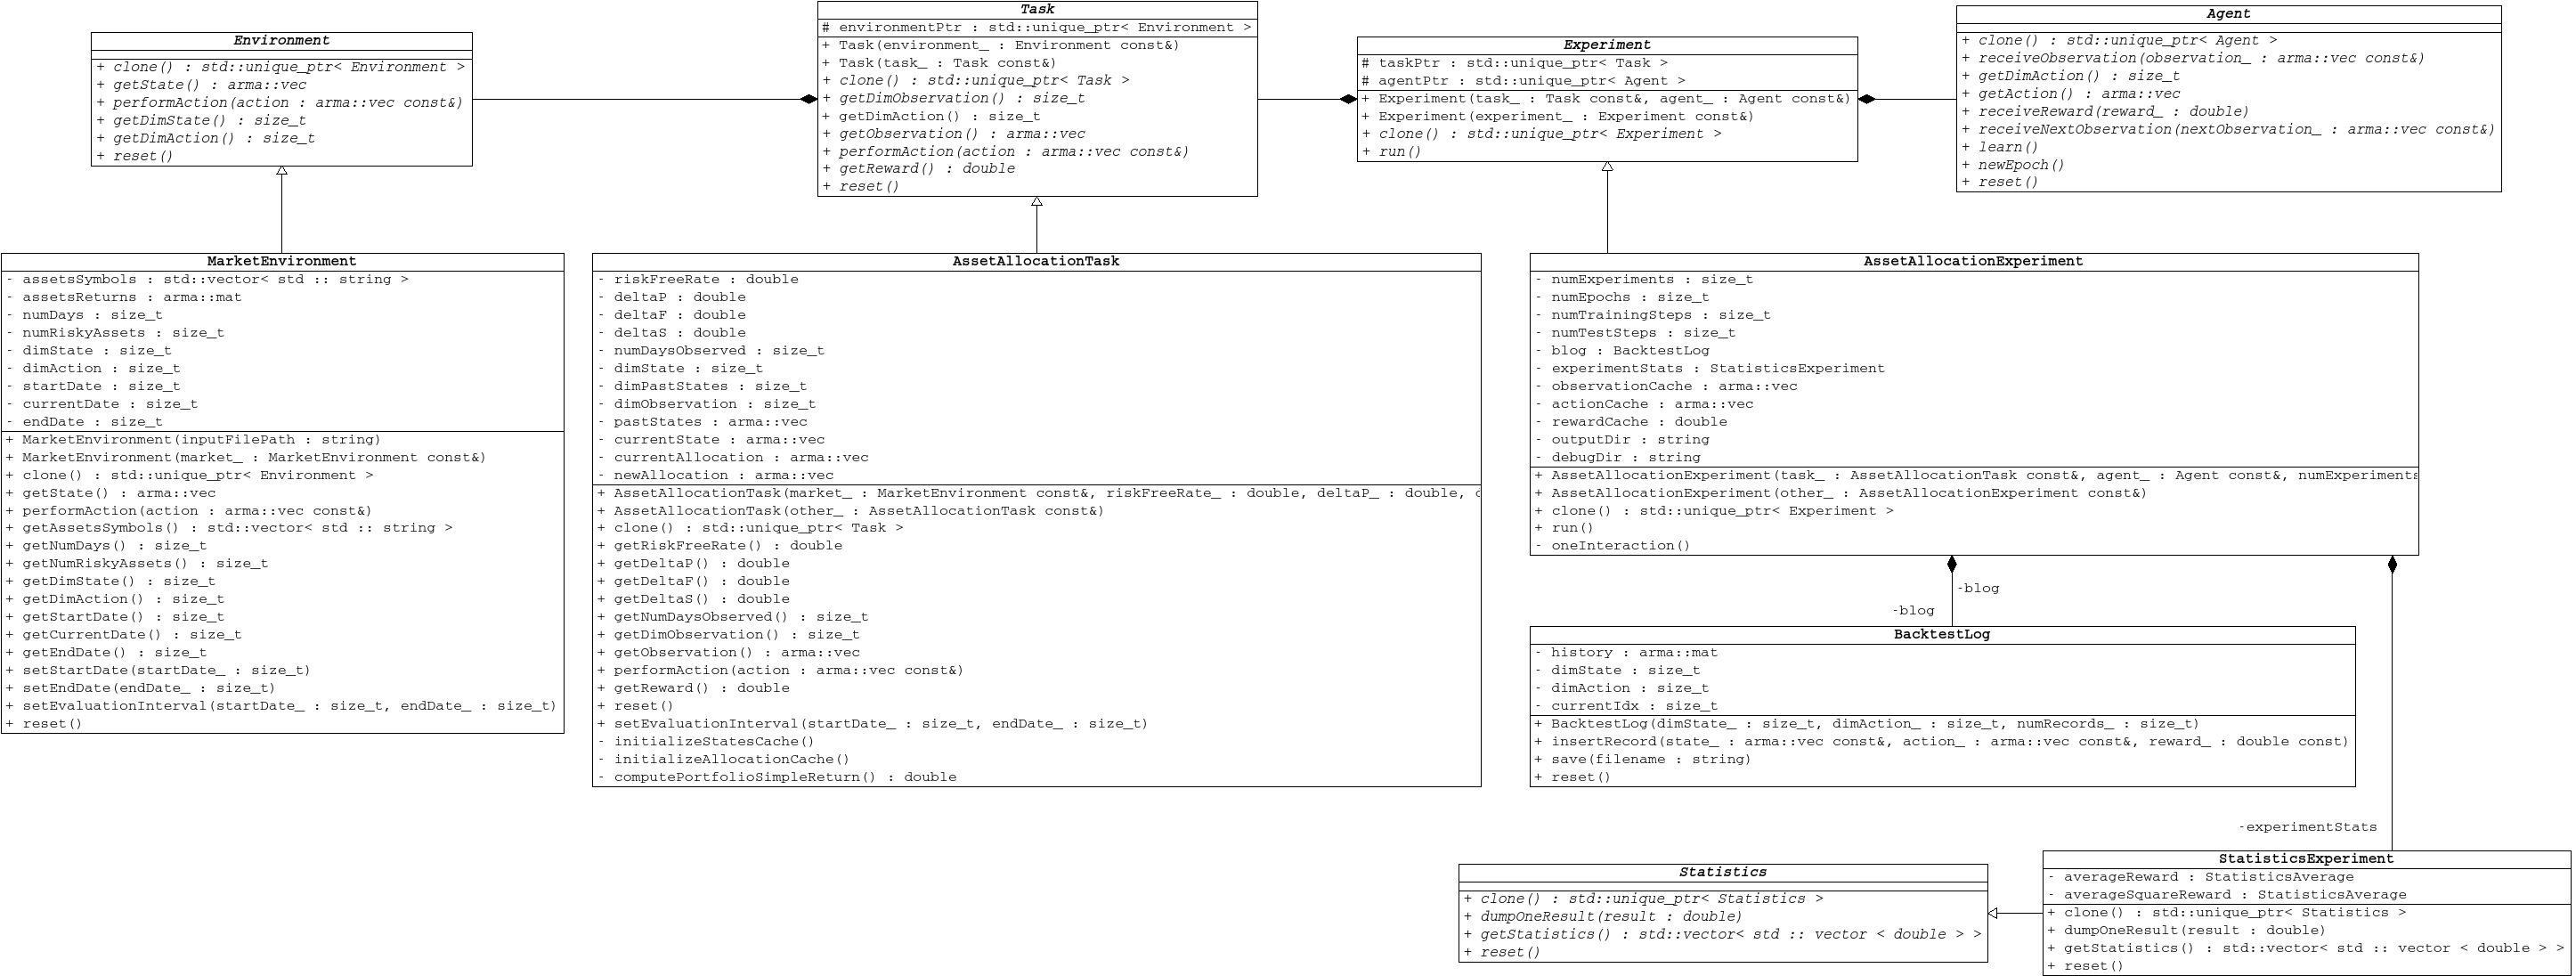
\includegraphics[width=\textwidth]{Images/agent_environment_interaction}
    \caption{Class architecture for the learning process in the asset allocation problem.}
    \label{fig:PropProf}
\end{figure}

\begin{sidewaysfigure}[ht]
    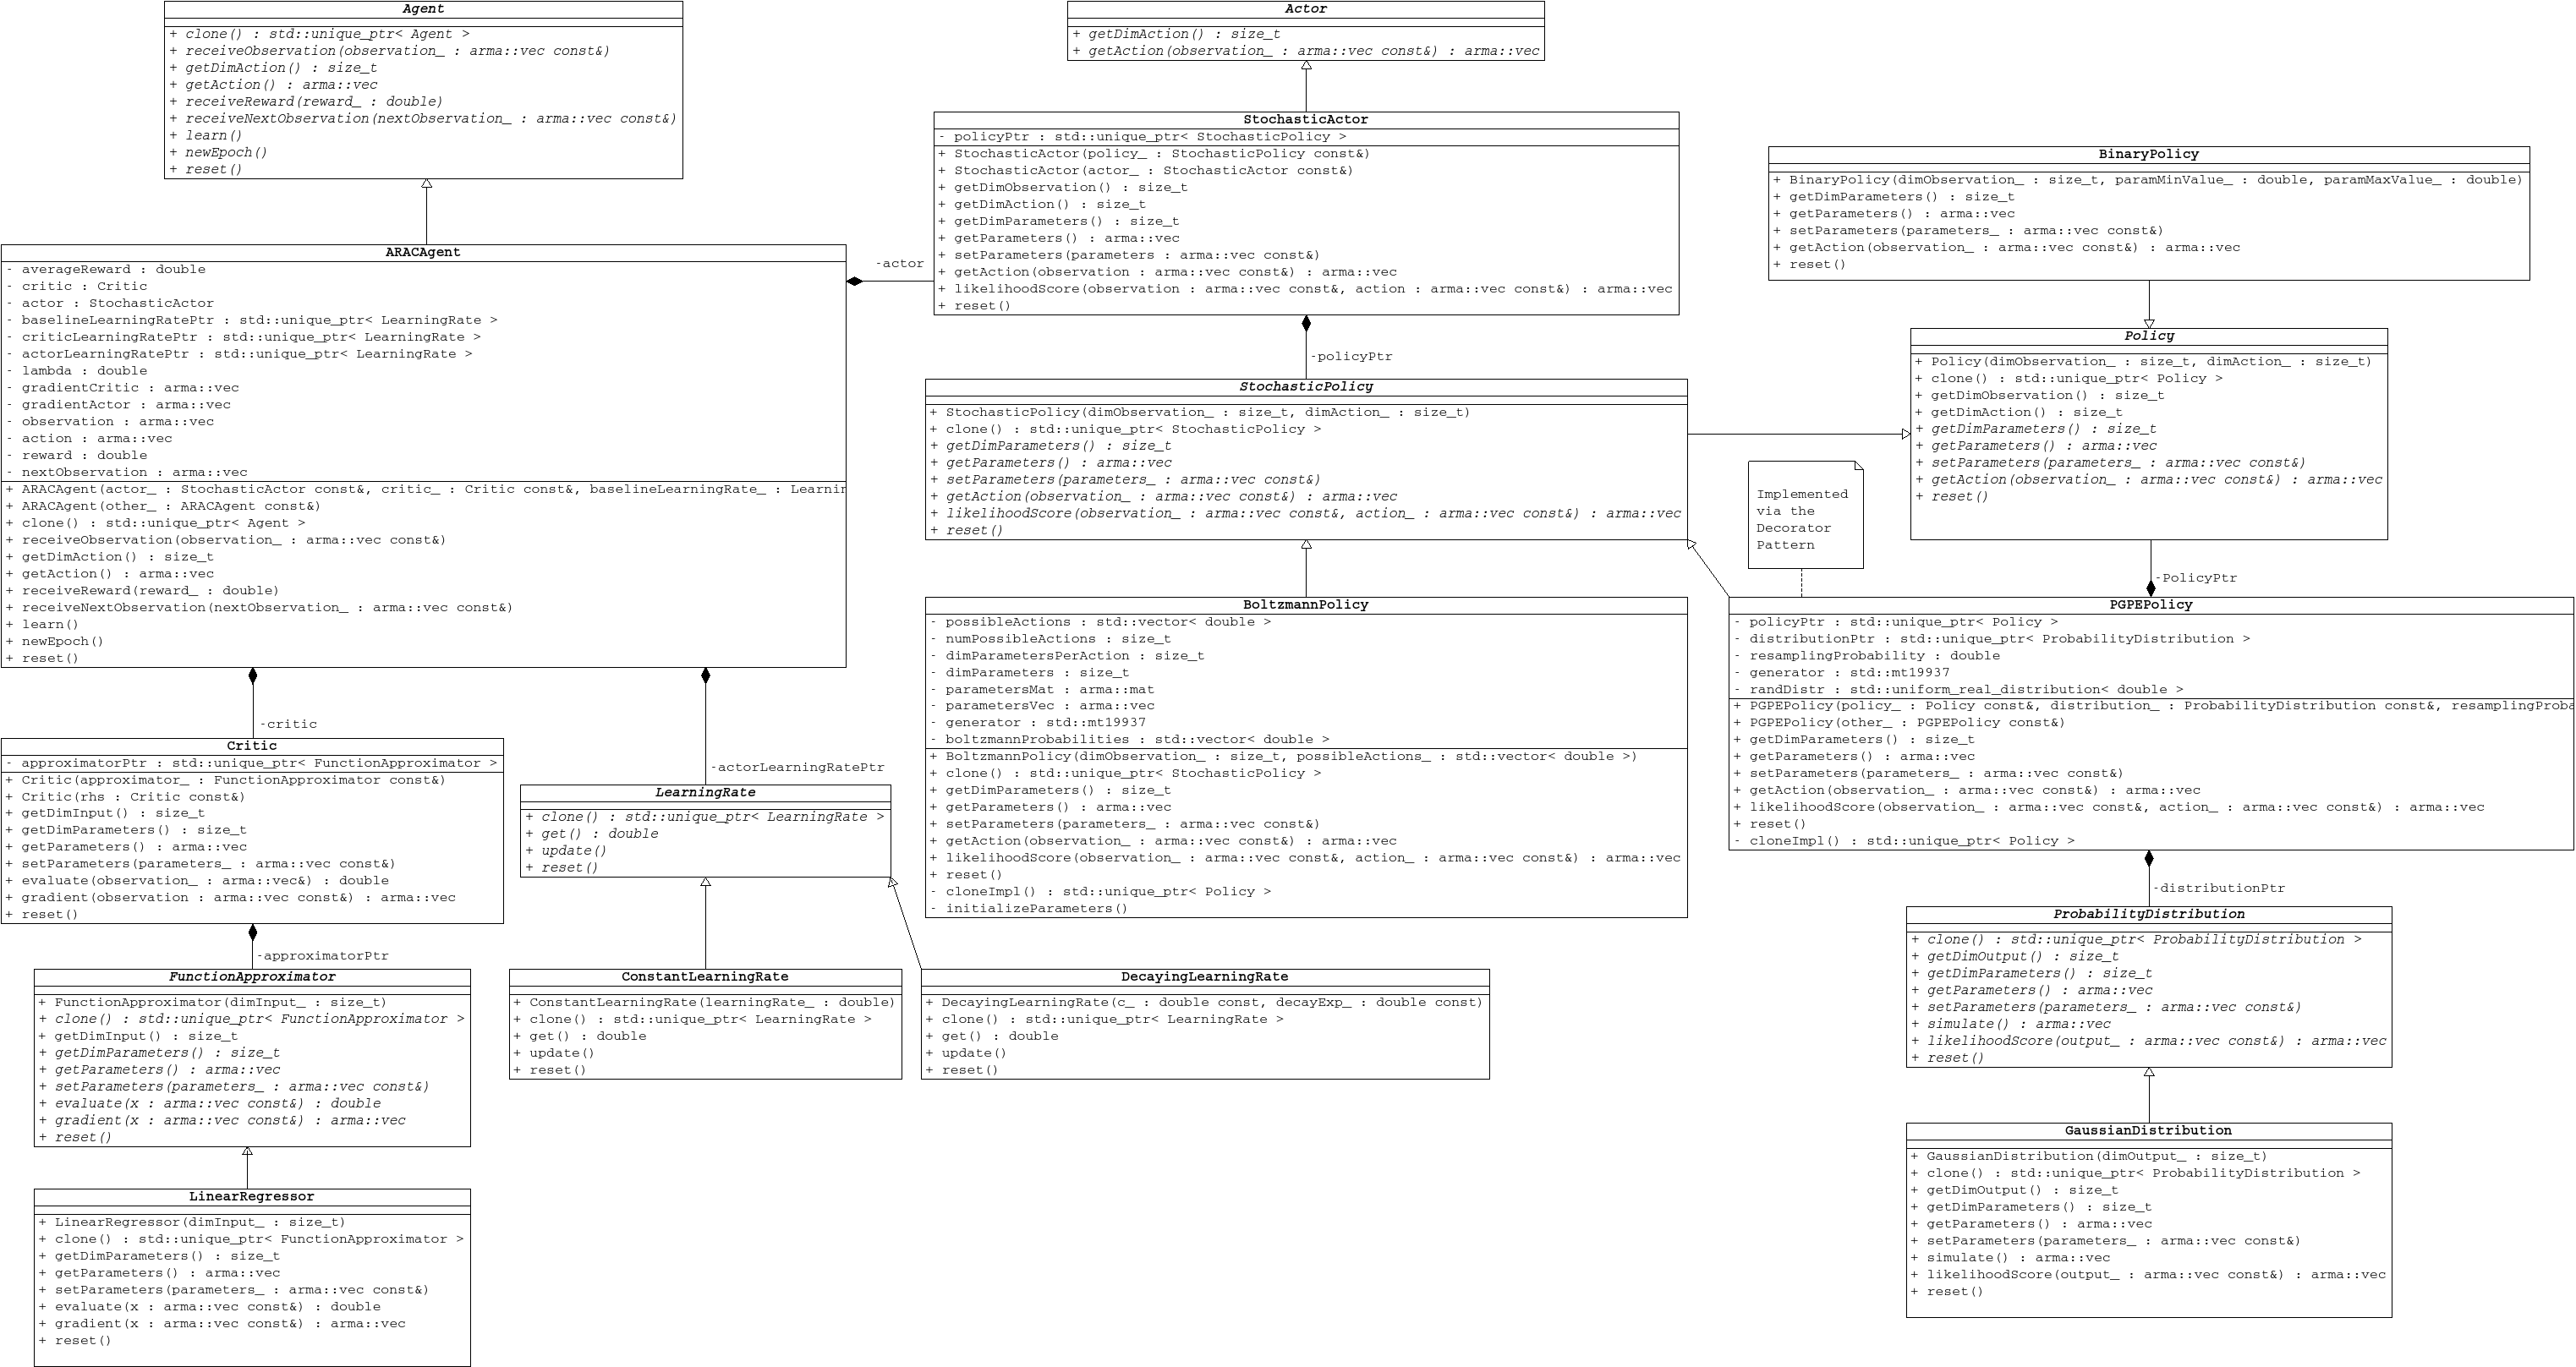
\includegraphics[width=\textwidth]{Images/agent}
    \caption{Class architecture for an Average Reward Actor-Critic agent (ARAC).}
    \label{fig:PropProf}
\end{sidewaysfigure}

\clearpage
\section{Execution Pipeline}
\label{sec:execution_pipeline}


\section{Numerical Results}
\label{sec:numerical_results}

In this section we present the numerical results of the online version of the policy gradient algorithms discussed in Section \ref{sec:basics_reinforcement_learning} for the asset allocation problem. 

\subsection{Synthetic Asset}
To assess the different reinforcement learning methods in a controlled environment, the learning algorithms are tested on a synthetic asset, which whose behavior presents some features that can be traded profitably. We simulated the log-price series $\{z_t\}$ for the risky asset as a random walk with autoregressive trend $\{\beta_t\}$. The two-parameter model is thus given by
\begin{equation}
	\begin{split}
		z_t &= z_{t-1} + \beta_{t-1} + \kappa \epsilon_t\\
		\beta_t &= \alpha \beta_{t-1} + \nu_t\\
	\end{split}
\end{equation}
We then define the synthetic price series as
\begin{equation}
	Z_t = \exp\left(\frac{z_t}{\max_t z_t - \min_t z_t}\right)
\end{equation}
This model is often taken as a benchmark test in the automated trading literature, see for instance \cite{moody1998performance}. In addition to presenting some exploitable patterns, the model is stationary and therefore the policy learned on the training set should generalize well on the test set, also known as backtest in the financial jargon. Thus we would expect our learning algorithms to perform well on this test case. 

\subsection{Experimental Setup}   
All the algorithms were tested on the same price series of size $9000$, generated from the process described above using $\alpha = 0.9$ and $\kappa = 3$. The learning process consisted of $500$ training epochs on the first $7000$ days of the series with a learning rate that decreased at each epoch according to a polynomial schedule. The trained agents were subsequently backtested on the final $2000$ days, during which the agents kept learning online in order to try to adapt to the changing environment. The results that we present are the average of $10$ independent experiments that used slightly different random initialization of the policy parameters.   

\subsection{Convergence}
Let us first discuss the case with no transaction costs. Figure \ref{fig:single_synthetic_neutral_convergence} shows the learning curves for the three risk-neutral algorithms in terms of average daily reward, which is the quantity being maximized by the algorithms, the daily reward standard deviation and the annualized Sharpe ratio. The first thing we observe is the ARAC algorithm seems not to be improving the trading strategy as the training epochs go by. The average reward obtained is close to zero and will be surely be negative once transaction costs are introduced. On the other hand, NPGPE slowly converges to a profitable strategy which is however suboptimal compared to the one found by PGPE, that is better in all three measures considered. It is interesting to notice that PGPE and NPGPE yield a learning curve for the Sharpe ratio very similar to the one for the average reward. Even if the algorithm is risk-neutral, it manages to improve a risk-senitive measure at the same time of the average reward. This might be simply a peculiarity of the very simple model assumed for the synthetic risky asset. Moreover, since the price process is stationary, the trading strategy learned on the training set perfectly generalizes to the test set. 
\begin{figure}[t!]
	\centering
	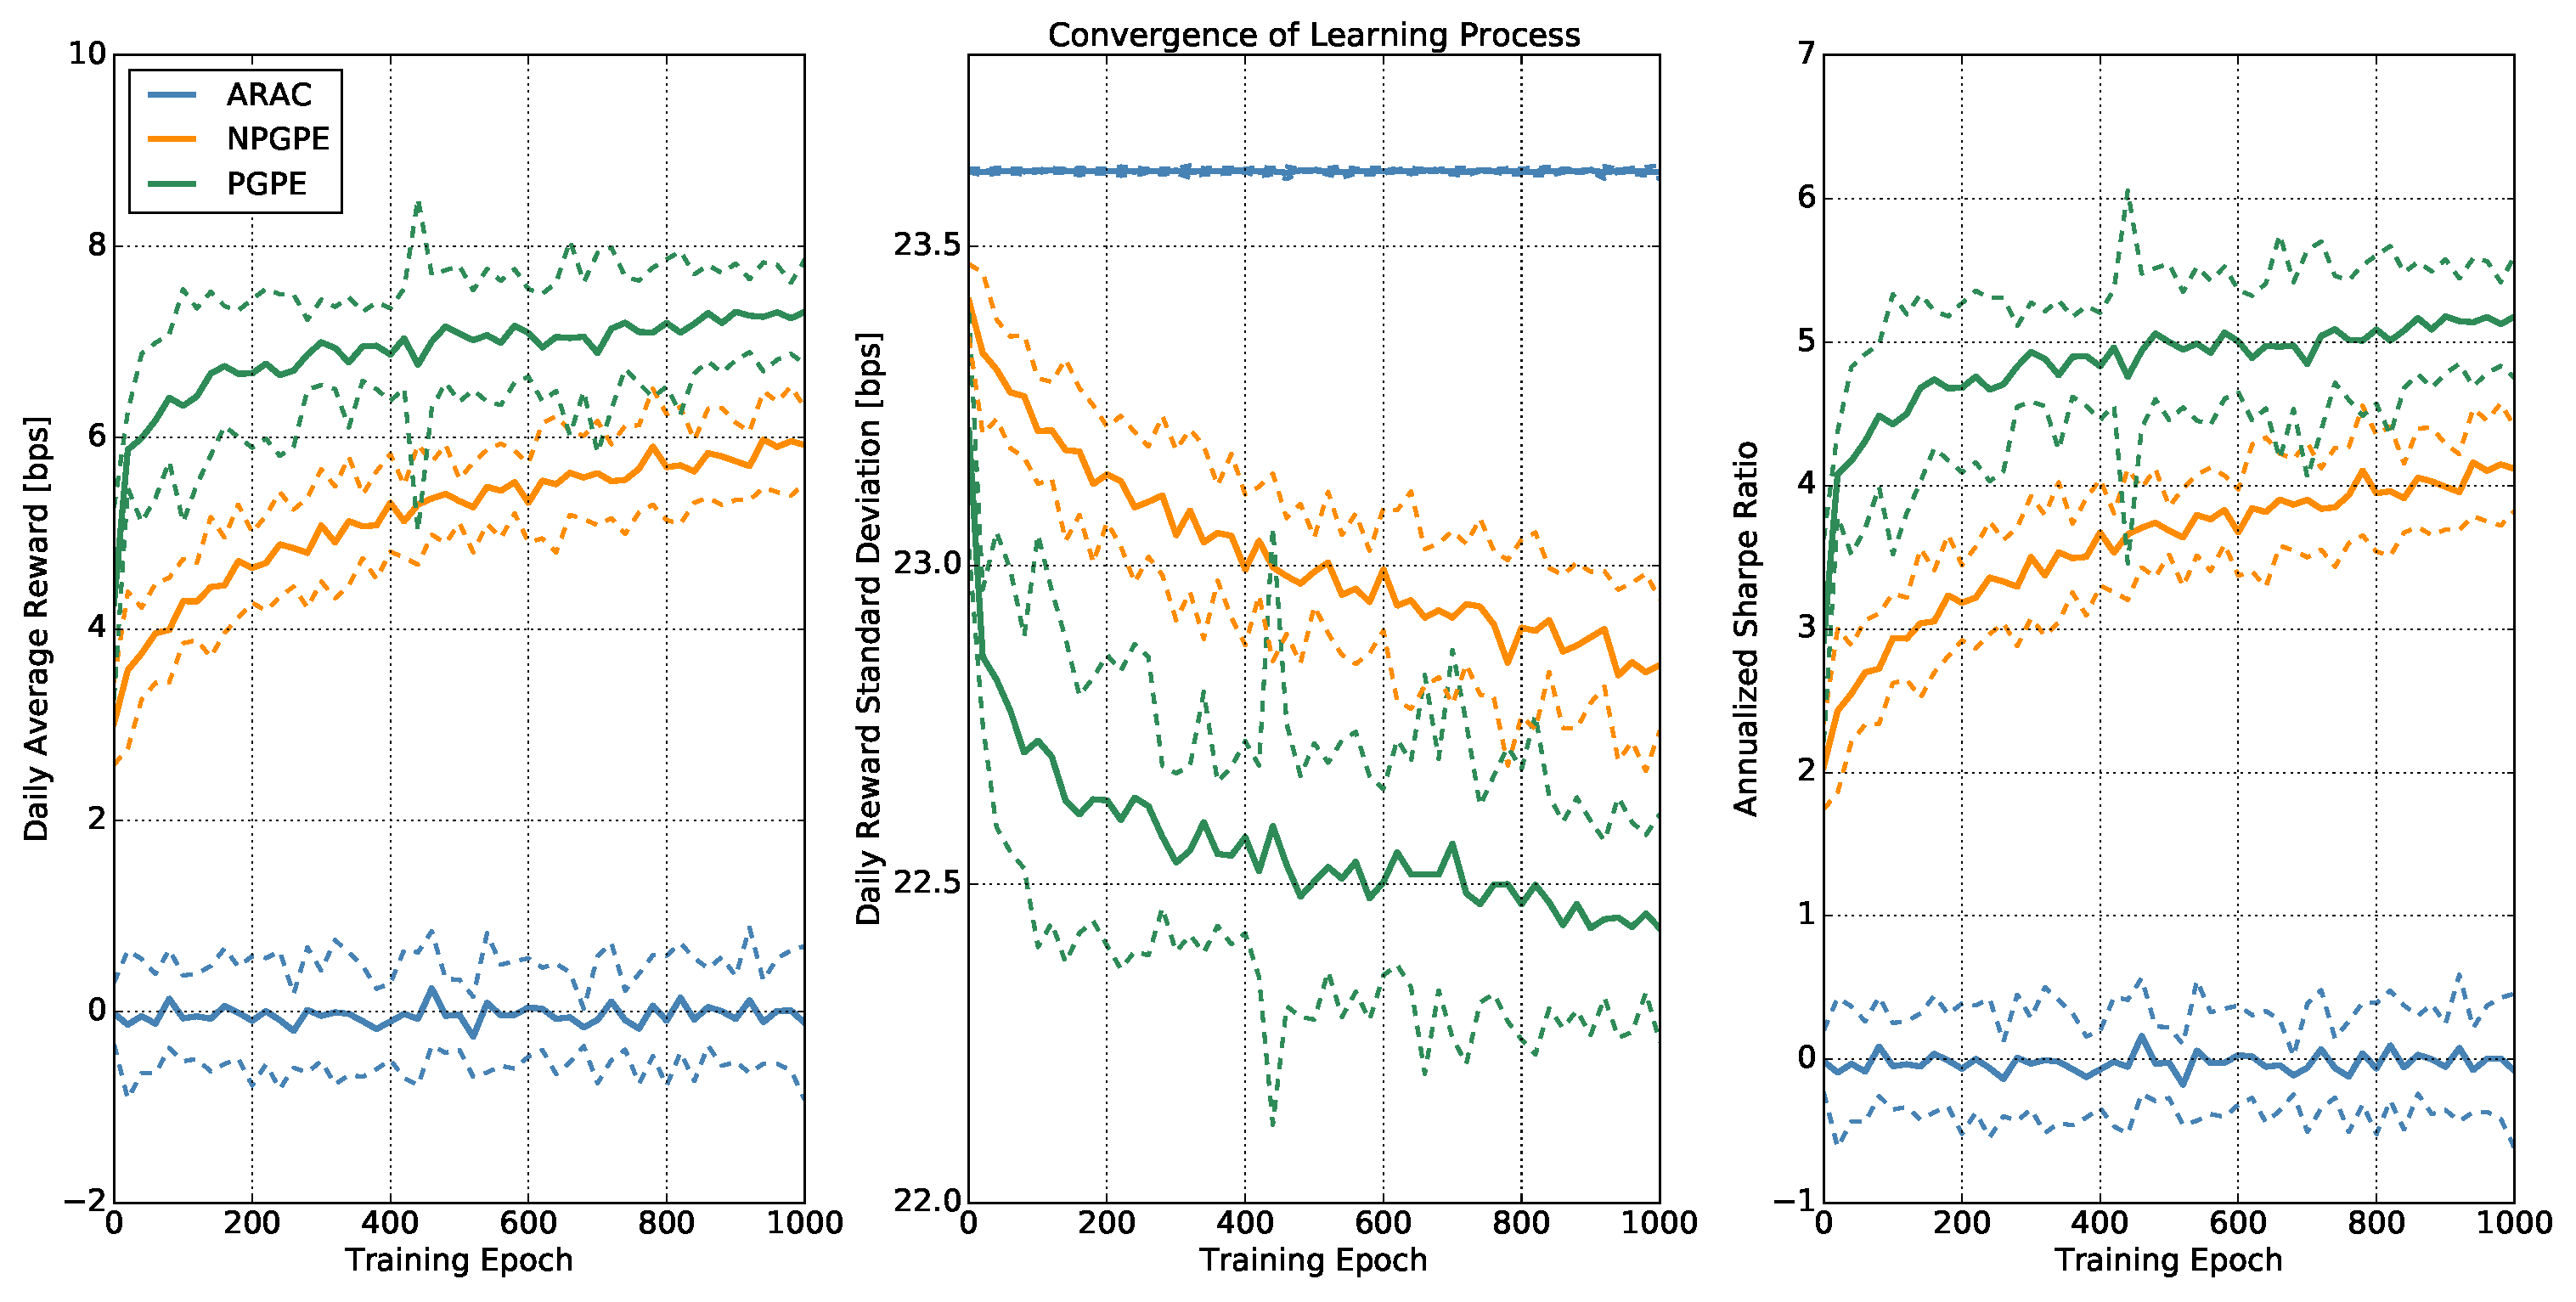
\includegraphics[height=6cm,width=1.0\textwidth]{Images/6_0_single_synthetic_neutral_convergence}
	\caption[Risk-neutral learning process for one synthetic risky asset]{Risk-neutral learning process for the asset allocation problem with one synthetic risky asset.}
	\label{fig:single_synthetic_neutral_convergence}
\end{figure}

\subsection{Performances}
Figure \ref{fig:single_synthetic_neutral_performance} compares the backtest performances of the three learned policies and a Buy and Hold strategy, which simply consists in investing all the available capital in the risky asset. Let us repeat that the solid lines are the averages of $10$ independent experiments, which allows us to determine the $95\%$ confidence intervals represented with the dashed lines. We clearly see that NPGPE and PGPE easily beat the market, realizing a total profit of $231.63\%$ and $314.34\%$ respectively against the $7.81\%$ profit of the Buy and Hold strategy over the same period. More statistics of the trading strategies are reported in Table \ref{tab:single_synthetic_neutral_performance}.
\begin{figure}[t]
	\centering
	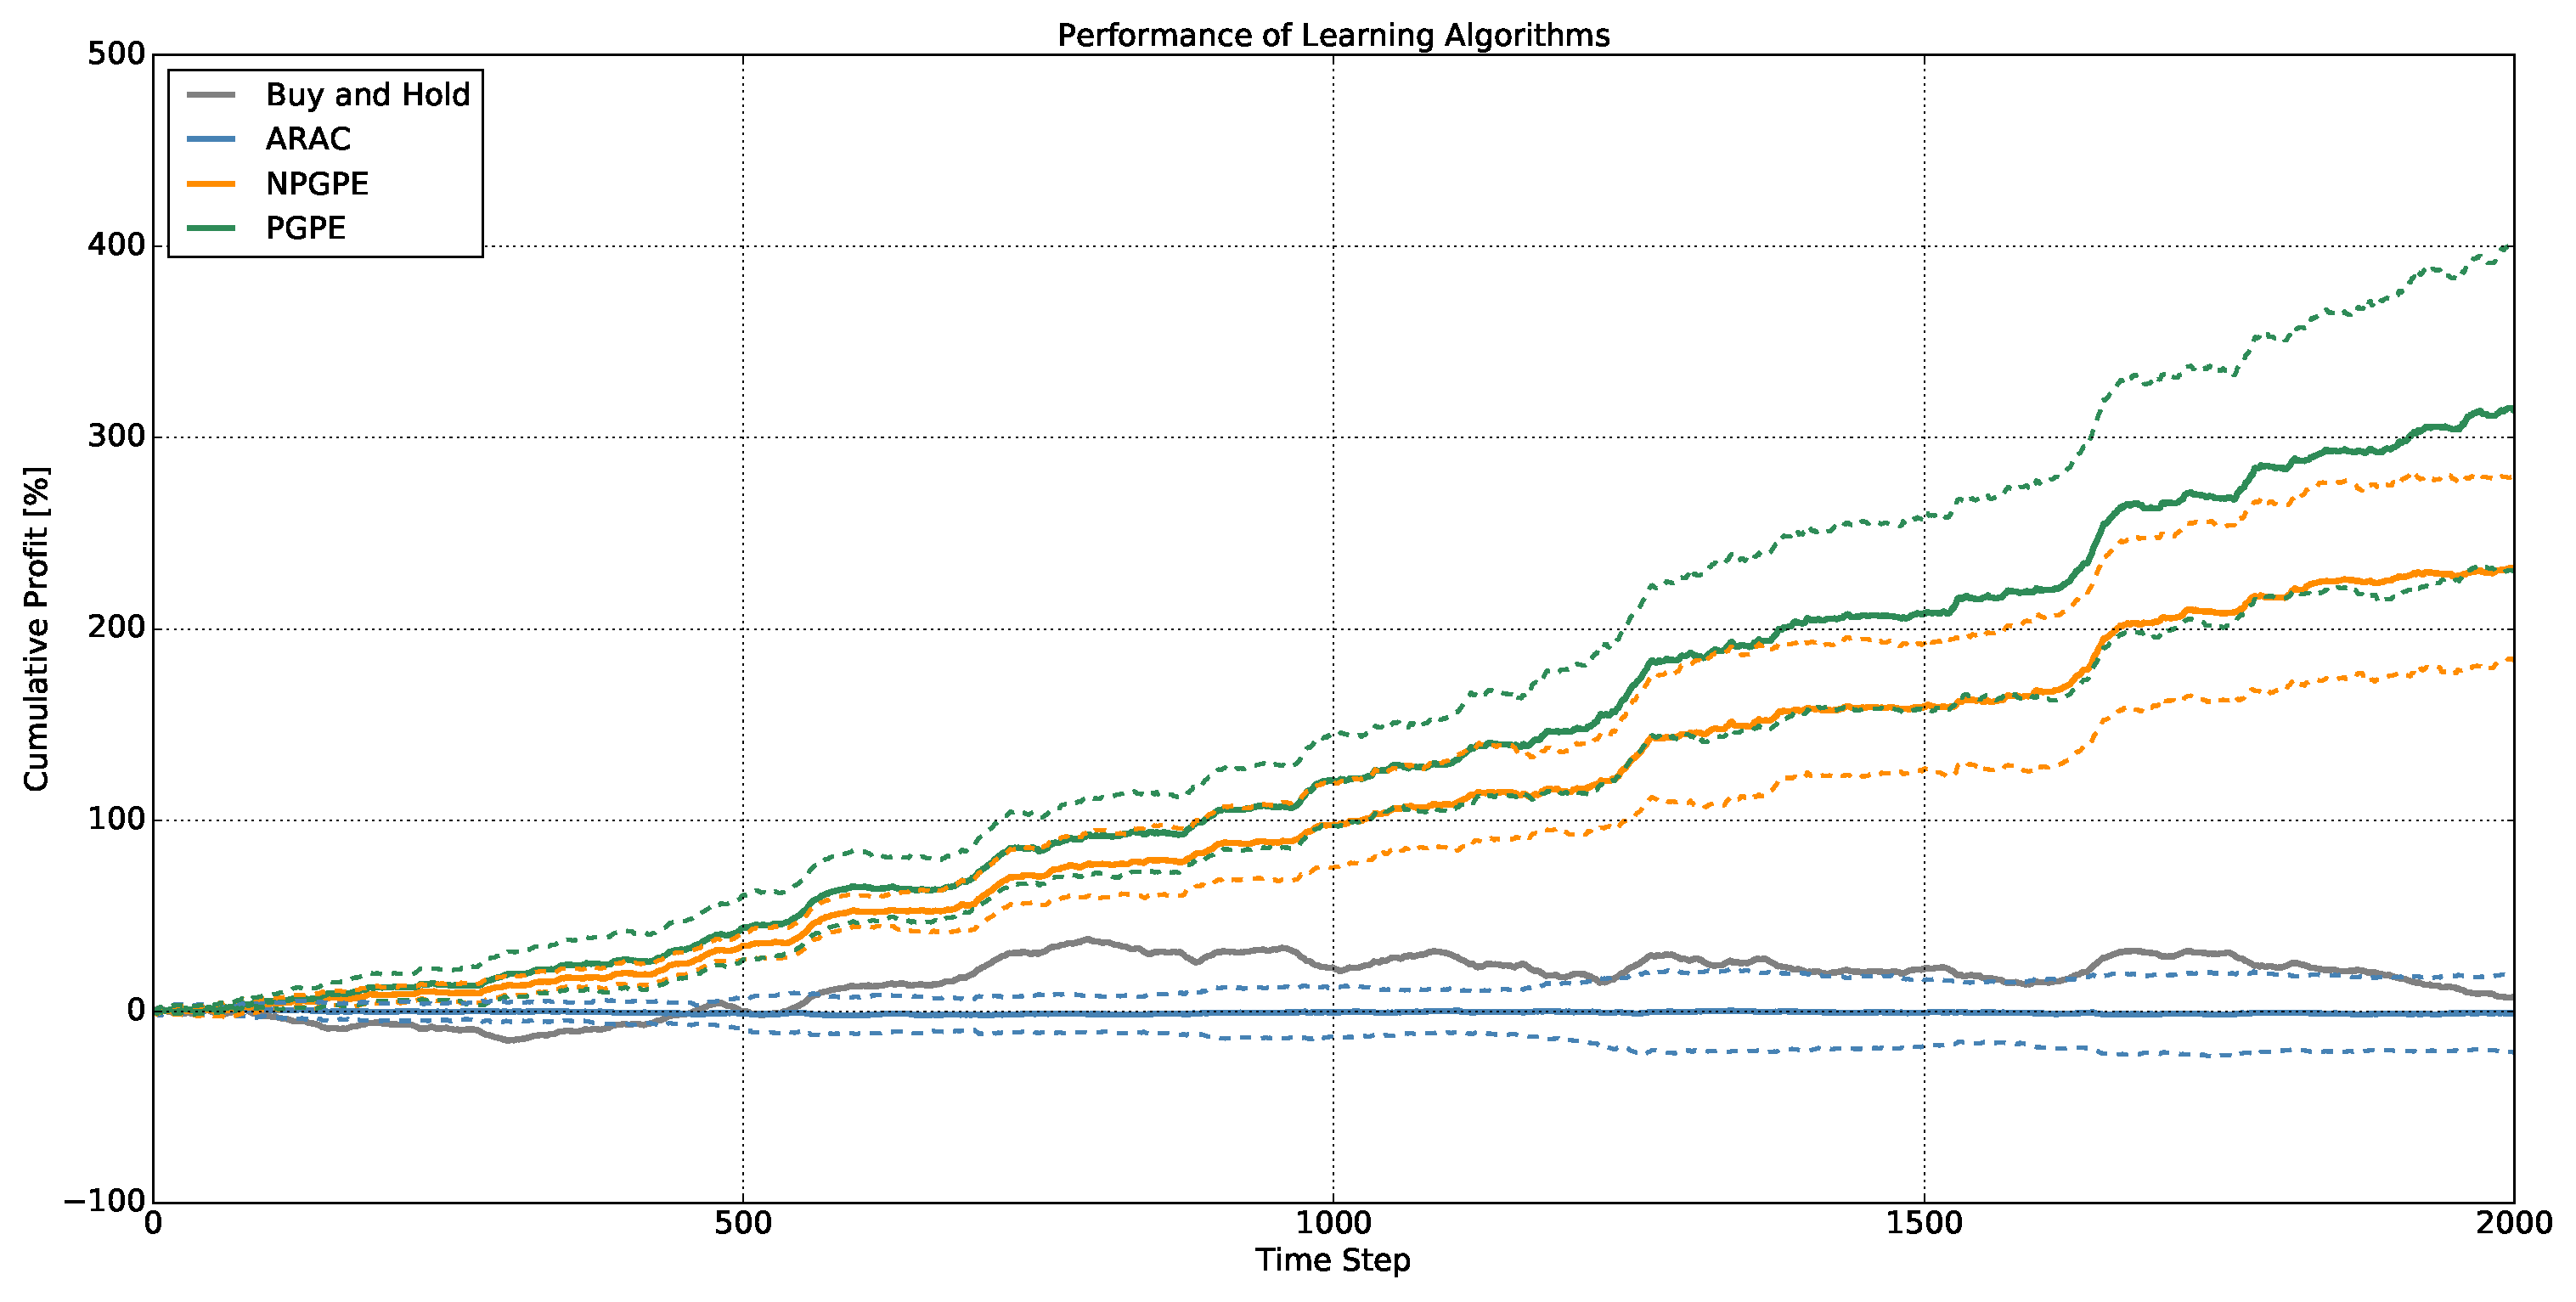
\includegraphics[height=6cm,width=1.0\textwidth]{Images/6_1_single_synthetic_neutral_performance}
	\caption[Backtest performance with one synthetic risky asset]{Backtest performance of trained trading systems for the asset allocation problem with one synthetic risky asset.}
	\label{fig:single_synthetic_neutral_performance}
\end{figure}
\begin{table}[t!]
\centering
\begin{tabular}{@{}lllll@{}}
\toprule
 & \multicolumn{1}{c}{Buy and Hold} & \multicolumn{1}{c}{ARAC} & \multicolumn{1}{c}{NPGPE} & \multicolumn{1}{c}{PGPE} \\ \midrule
Total Return & 7.81\% & -0.86\% & 231.63\% & 314.34\% \\
Daily Sharpe & 0.27 & -0.02 & 4.13 & 4.95 \\
Monthly Sharpe & 0.19 & -0.07 & 2.90 & 3.26 \\
Yearly Sharpe & 0.23 & -0.10 & 1.55 & 1.76 \\
Max Drawdown & -22.35\% & -12.60\% & -3.72\% & -3.27\% \\
Avg Drawdown & -1.75\% & -1.81\% & -0.49\% & -0.43\% \\
Avg Up Month & 2.87\% & 1.14\% & 2.47\% & 2.74\% \\
Avg Down Month & -2.58\% & -1.10\% & -0.73\% & -0.67\% \\
Win Year \% & 40.00\% & 44.00\% & 98.00\% & 100.00\% \\
Win 12m \% & 56.36\% & 48.00\% & 100.00\% & 100.00\% \\
Reallocation Freq & 0.00\% & 50.01\% & 19.99\% & 15.43\% \\
Short Freq & 0.00\% & 50.13\% & 41.59\% & 44.25\% \\ \bottomrule
\end{tabular}
\caption[Backtest statistics for risk-neutral learning with one synthetic risky asset]{Backtest statistics of the risk-neutral trading strategies for the asset allocation problem with one synthetic risky asset.}
\label{tab:single_synthetic_neutral_performance}
\end{table}

\subsection{Impact of Transaction Costs}
In the algorithmic trading literature there are many examples of strategies based on the prediction of future rewards starting from more or less complex indicators \cite{kamijo1990stock}, \cite{saad1998comparative}, \cite{liang2011stock}. However, as pointed out in \cite{deng2016deep}, the performances of these methods quickly degrade when transaction costs for changing the portfolio composition or for shorting a security
are considered. Indeed, these methods simply invest based on the prediction of the future returns, without explicitly taking into account transaction costs. On the other hand, reinforcement learning algorithms should learn to avoid frequent reallocations or shorts thanks to the feedback mechanism between the learning agent and the system, thus generating better trading performances. In this section we analyze how the strategies learned by PGPE and by NPGPE change when gradually increasing the proportional transaction costs and the short-selling fees. Intuitively, we expect a progressive reduction of the frequency of reallocation and of shorting the risky asset.\\
Figure \ref{fig:impact_transaction_costs} shows the impact of proportional transaction costs on the trading strategies learned by PGPE and by NPGPE. As expected, the frequency of reallocation for both strategies quickly drops to zero as the transaction costs increase, converging to the profitable buy and hold strategy. It is peculiar that the reallocation frequency for the PGPE strategy initially drops more quickly than for the NPGPE strategy, but then slows down and even increases when $\delta_P = 20$ bps.
In summary, both algorithms are able to identify reallocation as the cause for lower rewards and to subsequently reduce the rate of reallocation, converging towards the simple yet profitable buy and hold strategy. Figure \ref{fig:impact_short_selling_fees} shows the impact of short-selling fees on the trading strategies learned by PGPE and NPGPE. Both algorithms behave as expected, displaying a progressive reduction of the frequency of short positions as the fees increase. For large values of short-selling fees, both strategies converge to the profitable buy and hold strategy, which completely avoids paying the fees. In particular, PGPE quickly replicates the buy and hold strategy. On the other hand, NPGPE is not able to exactly reproduce the buy and hold strategy but it seems to converge to it for very large values of the short-selling fee. 
\begin{figure}[t!]
	\centering
	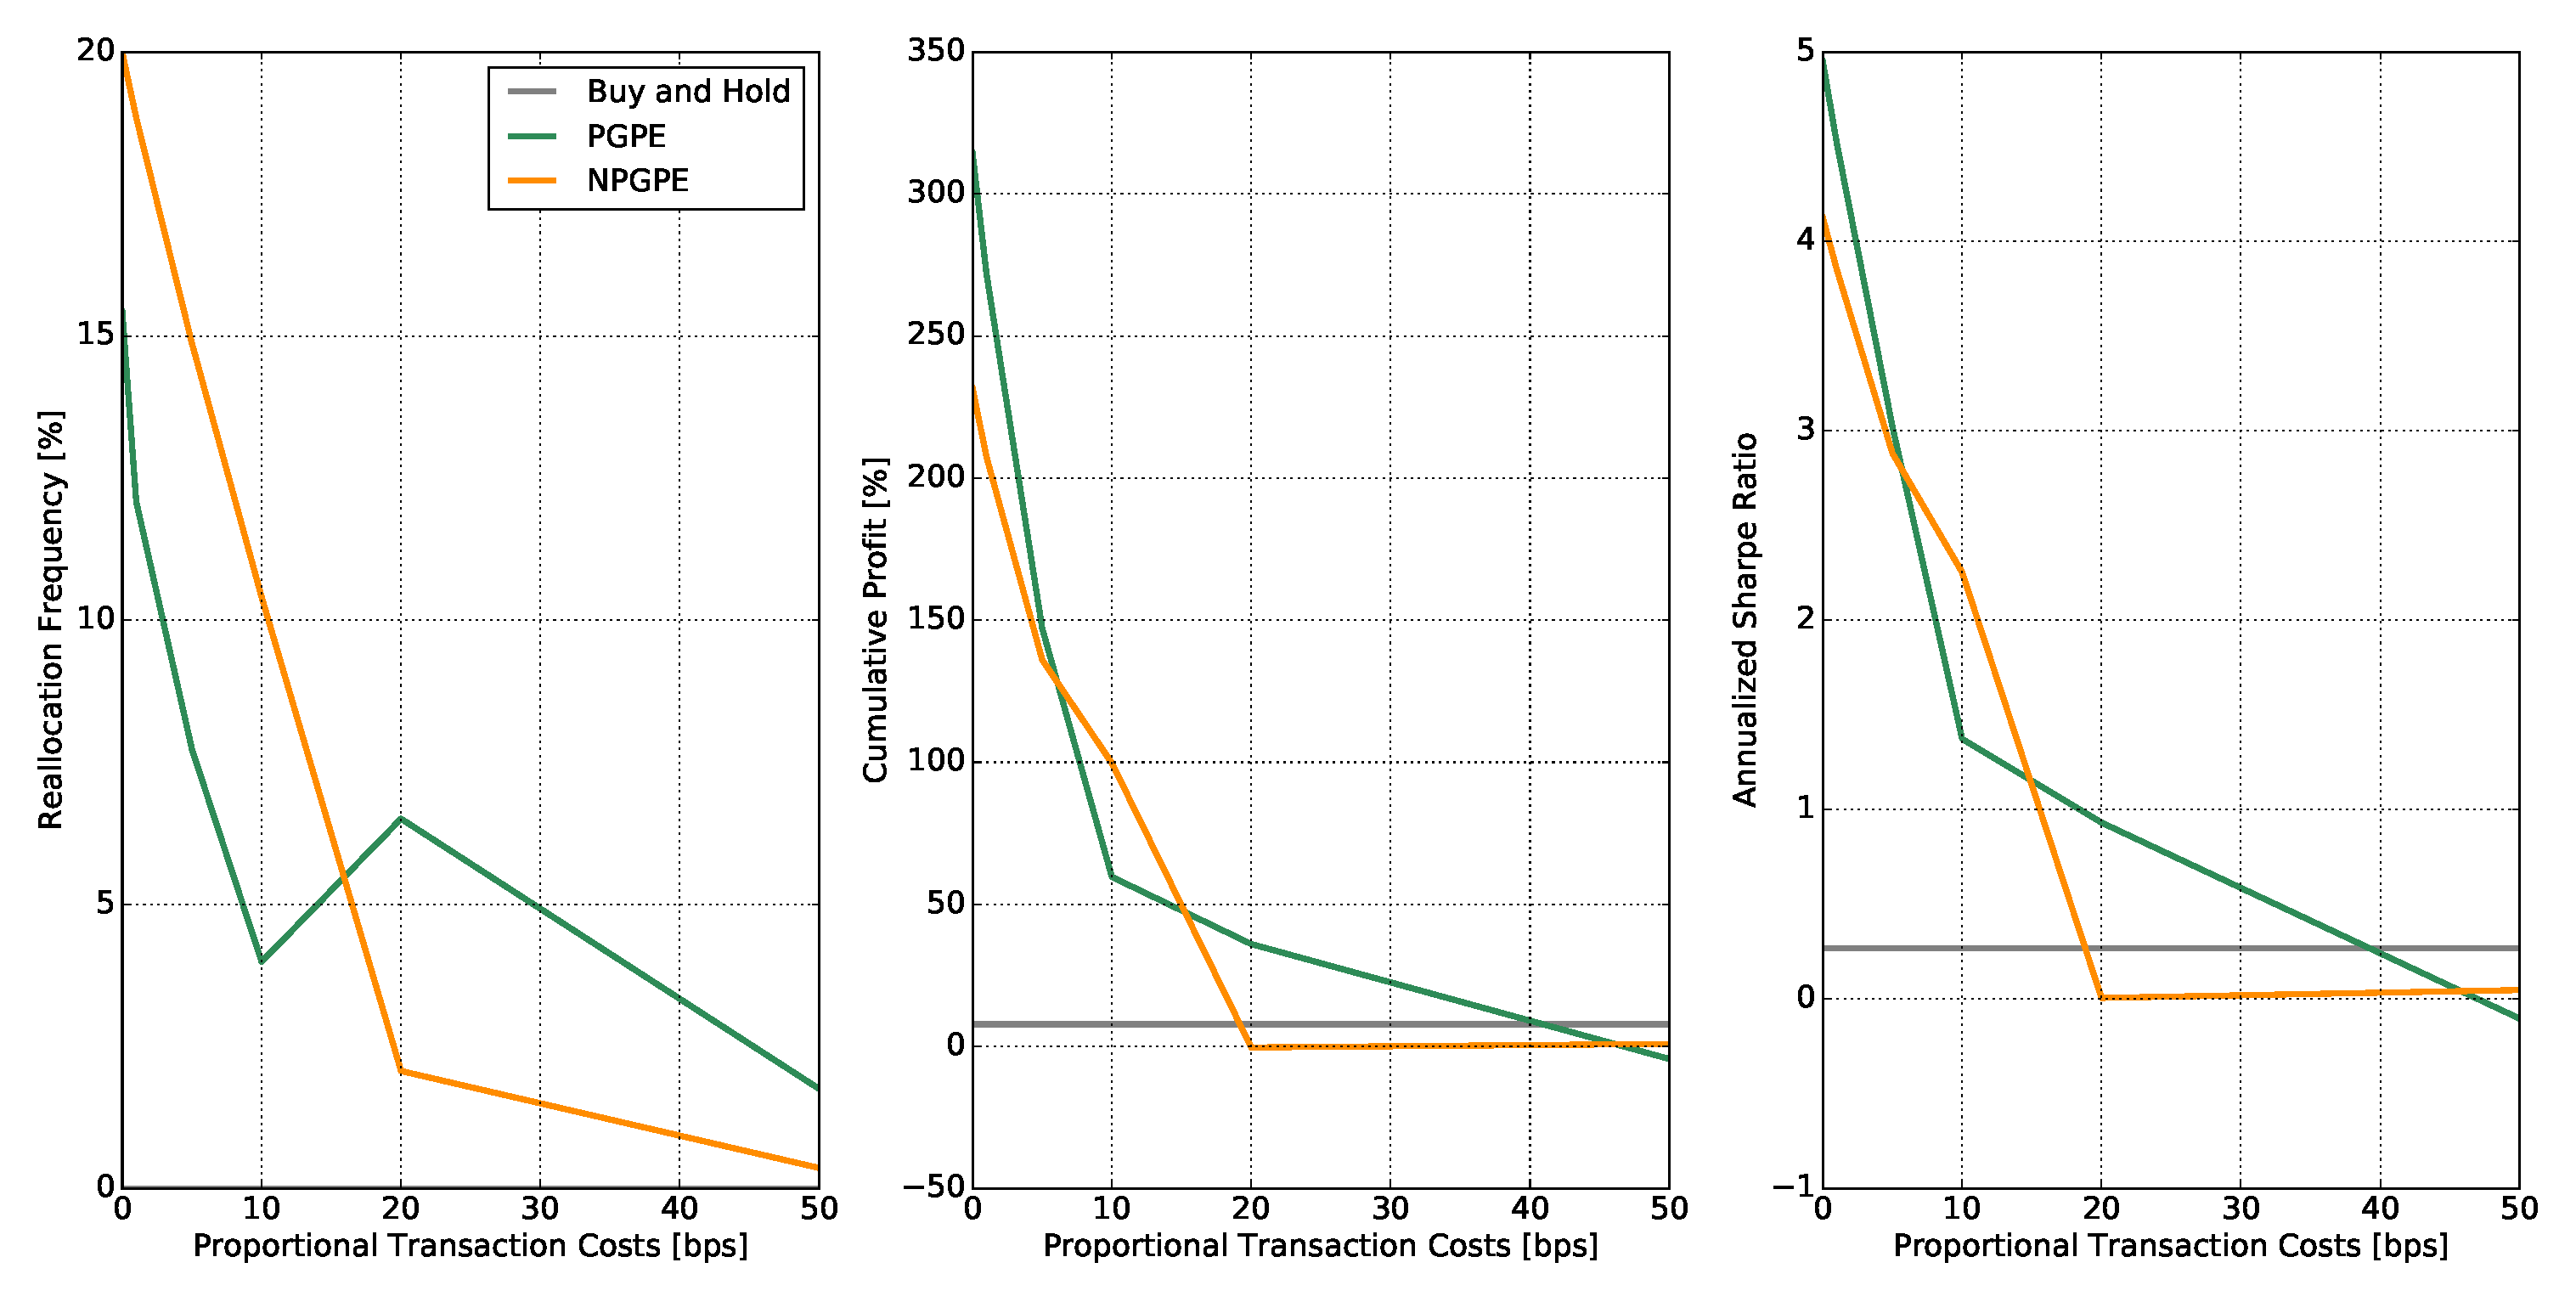
\includegraphics[height=6cm,width=1.0\textwidth]{Images/6_2_impact_transaction_costs}
	\caption[Impact of proportional transaction costs]{Impact of proportional transaction costs on the trading strategies learned by PGPE and NPGPE.}
	\label{fig:impact_transaction_costs}
\end{figure}

\begin{figure}[t!]
	\centering
	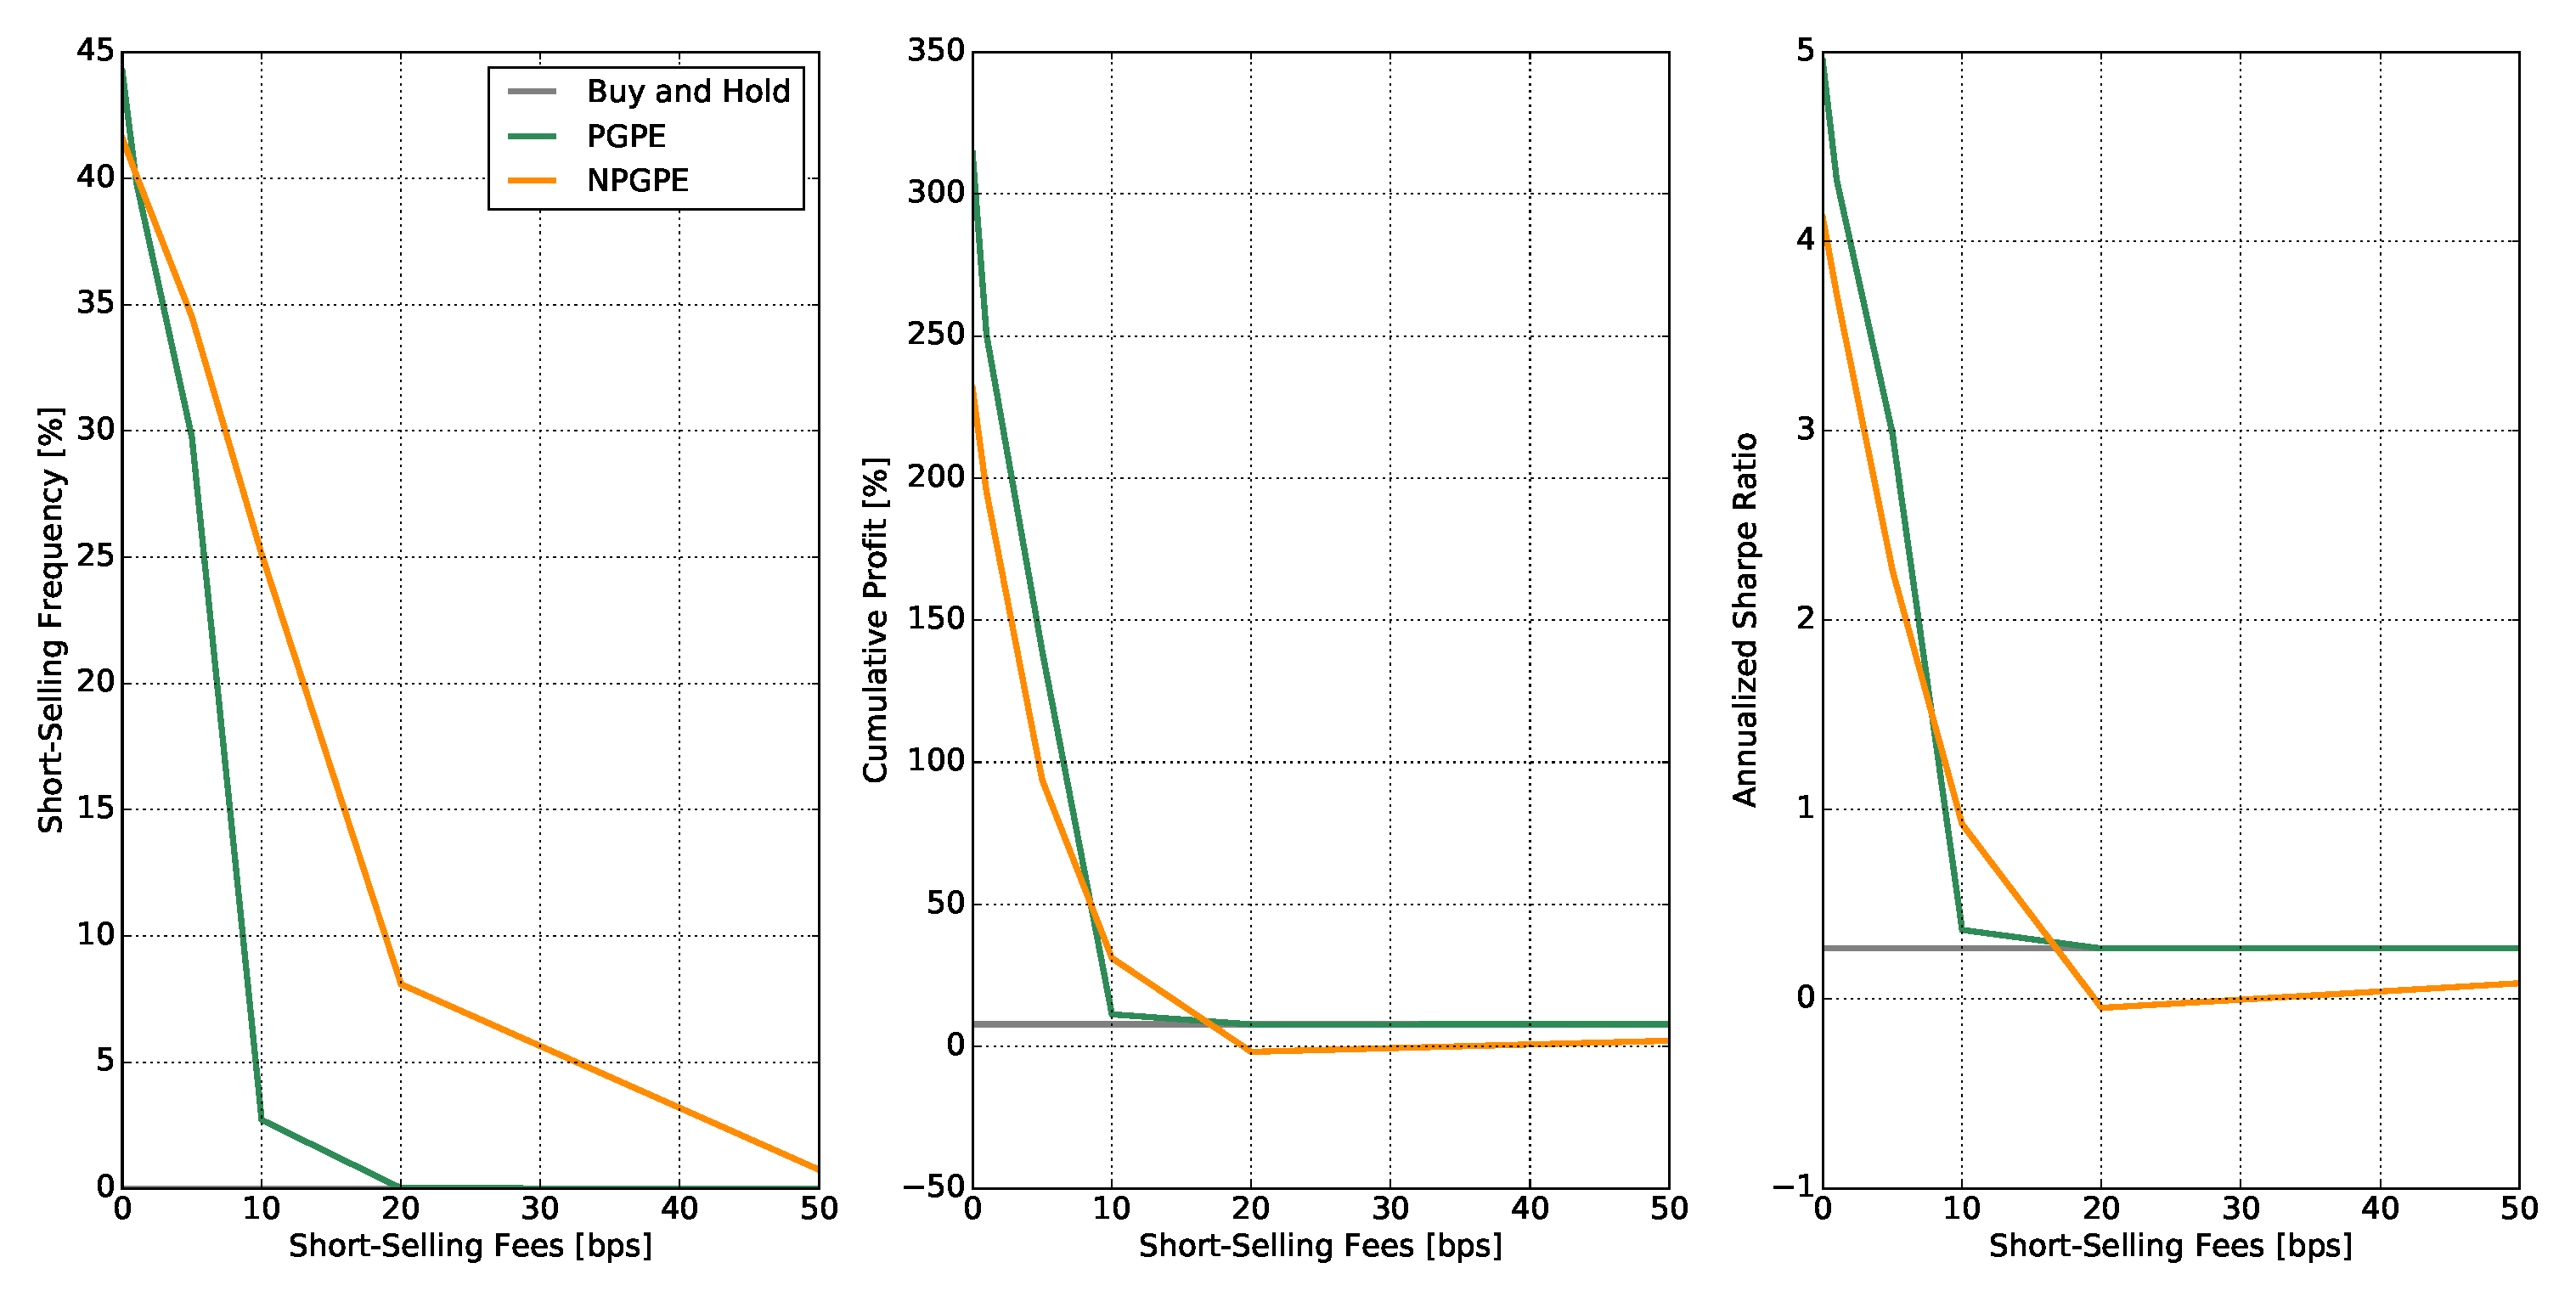
\includegraphics[height=6cm,width=1.0\textwidth]{Images/6_3_impact_short_selling_fees}
	\caption[Impact of short-selling fees]{Impact of short-selling fees on the trading strategies learned by PGPE and NPGPE.}
	\label{fig:impact_short_selling_fees}
\end{figure}
\section{Conclusion}
\label{sec:conclusion}



\subsubsection*{Acknowledgments}

TODO

\clearpage
\bibliographystyle{unsrt}
\bibliography{Bibliography/bibliography}


\end{document}